\section{Charged comparison and the numerical inequality}\label{cp:section}

We first fix one strict rest exterior supplied by
Proposition~\ref{en:rest-preparation}.  In this section $g,K,\EE,\BB$
denote these prepared data, $E_*$ is their ADM energy, and their ADM
momentum is zero.  The tensor $K$ has compact support.  The end has the
strong metric and field decay required below, and, with the geometric
density conventions of Definition~\ref{def:data},
\begin{equation}\label{cp:strict-margin}
 D_g(Y):=\mu+J(Y)-I_g(Y)>2\rho,
 \qquad |Y|_g\le1,\qquad \rho=c_*r^{-3-\beta}>0,
\end{equation}
where
\[
 I_g(Y)=|\EE|_g^2+|\BB|_g^2+2(\EE\times\BB)\cdot Y,
 \qquad 0<\beta<1.
\]
On each boundary component a fixed sign $\sigma_i\in\{1,-1\}$ satisfies
$H+\sigma_i\operatorname{tr}_S K<0$.  The argument treats these signs
component by component.

Fix $0<\epsilon<1$.  We use the filled manifold $\Omega_N$, its
background metric $g_N$, and all the quantities of
Section~\ref{sy:section}; thus $g_N=g$ on the original exterior.
The dimension is three and $k=2$.  In particular,
\begin{equation}\label{cp:parameters}
 \ell=e^{-N\epsilon},\qquad \eta=\ell^{3/2},\qquad h=\eta f,
 \qquad \bar g=g_N+l^2df^2,
 \qquad \widehat g=e^{2t}\bar g.
\end{equation}
At each $N$ we first exhaust the outer Dirichlet boundary as in
Theorem~\ref{so:filled-solver}.  Every assertion below concerns the
resulting smooth solution on $\Omega_N$.  A symbol $\mathcal P_N$
denotes a positive polynomial bound in $1+N$, whose coefficients may
depend on this prepared exterior and on $\epsilon$.  Different
occurrences may denote different such bounds.

The quantitative inputs from Lemma~\ref{es:height} and
Proposition~\ref{es:distortion} are
\begin{equation}\label{cp:quantitative-inputs}
 \begin{gathered}
 -\epsilon<t\le Z\le\mathcal P_N,\qquad
 \ell\le l\le e,\qquad
 |f|+|df|_{g_N}\le e^{\mathcal P_N},\\
 |h|\le C,\qquad |h|\le Cr^{-b_1}\ \hbox{on the end},
 \qquad \frac34<b_1<1.
 \end{gathered}
\end{equation}
The constants in the height bounds are independent of $N$.
The filled backgrounds have uniform local geometry, and the volume of
their enlarged compact part is $O(1+N)$.  Higher derivative estimates
will only be used with $N$ fixed.

\subsection{The end flux and its small negative part}

\begin{lemma}[Mass cost of the filled deformation]\label{cp:mass-cost}
The metric $\widehat g$ has a well-defined ADM energy and
\begin{equation}\label{cp:mass-flux}
 E(\widehat g)=E_*-\frac{\mathfrak F_N}{8\pi},
 \qquad
 \mathfrak F_N=\int_{\Omega_N}u\Xi\,dV_{g_N}
 =\lim_{R\to\infty}\int_{r=R}g_N(V,\nu_R)\,dA_{g_N}.
\end{equation}
There is a nonnegative sequence $a_N$ such that
\begin{equation}\label{cp:mass-error}
 E(\widehat g)\le E_*+a_N,
 \qquad
 a_N\le\mathcal P_N(\ell+\ell^{1/2})\longrightarrow0.
\end{equation}
\end{lemma}

\begin{proof}
The end conclusion of Theorem~\ref{so:filled-solver} gives, at fixed
$N$, exponential decay of $f$ and each of its fixed-order derivatives,
and
\[
 t,Z=O_j(r^{-1}),\qquad t-Z=O_j(e^{-c_jr}),\qquad
 \Delta_g t=O(r^{-3-\beta}).
\]
Here the constants and the positive $c_j$ may depend on $N$.
Since $K=0$ sufficiently far out, $\mathcal T=O(r^{-4})$ up to
exponentially decaying terms, $u=1+O(r^{-1})$, and
$\eta a_w|df|$ decays exponentially.  For $N\epsilon>2$, the penalty
cutoff $m_0=\vartheta(N(t+\epsilon))$ vanishes sufficiently far out.
Consequently $u\Xi$ is absolutely integrable.  The divergence equation
and the absence of any boundary in $\Omega_N$ prove the flux identity
in Equation~\eqref{cp:mass-flux}.

The definition of $V$, $A_\chi=\Id+O_j(e^{-c_jr})$, and the same end
estimates show that
\[
 V=2\nabla t+O(r^{-3})+O(e^{-cr}).
\]
Thus its limiting flux is twice the limiting flux of $dt$.  The graph
term $l^2df^2$ makes no contribution to ADM energy.  Direct substitution
of $e^{2t}g$ into the ADM integral gives
\[
 E(e^{2t}g)-E(g)
 =-\frac1{4\pi}\lim_{R\to\infty}
       \int_{r=R}\partial_{\nu_R}t\,dA_g.
\]
The terms containing $(g-\delta)dt$, $t\,\partial g$, or $t\,dt$
have integrals $O(R^{-1})$; changing between Euclidean and $g$ normals
and measures has the same vanishing cost.  This proves the coefficient
and sign in Equation~\eqref{cp:mass-flux} without requiring a separately
chosen monopole coefficient for $t$.

It remains to estimate the possibly negative part of the integral.
Write $\sigma=|df|_{g_N}$.  On the support of $m_0$ the floor gives
$-\epsilon<t<-\epsilon+N^{-1}$, and therefore
$\ell\le l\le e\ell$ for large $N$.  Since $u=e^t l\sqrt D$ and
$D=1+l^2\sigma^2$, direct calculation gives
\begin{equation}\label{cp:penalty-weights}
 u\le C(\ell+\ell^2\sigma),\qquad
 uv\le C\ell^2\sigma,\qquad
 u a_w\sigma=e^tl^2\sigma^2\ge c\ell^2\sigma^2.
\end{equation}
The negative term in $u\Xi$ is consequently bounded in absolute value
by
\[
 \mathcal P_N\ell\rho_0
   +\mathcal P_N\ell^2\sigma(\rho_0+\rho_1).
\]
Young's inequality, using a fixed fraction of the positive
$\delta_0\eta u a_w\sigma$, bounds the second summand by
\[
 \frac{\delta_0\eta}{2}u a_w\sigma
     +\mathcal P_N\frac{\ell^2}{\eta}
                        (\rho_0^2+\rho_1^2).
\]
Here $\rho_0=r^{-3-\beta}$ and $\rho_1=r^{-2b_1}$.  Their required
integrals have polynomial bounds: the compact contribution is
$O(1+N)$, while on the end $\rho_0$, $\rho_0^2$, and $\rho_1^2$ are
integrable, the last because $4b_1>3$.  In particular, no integral of
$\rho_1$ is being assumed finite.  Positivity of $\mathcal T$, proved
in Proposition~\ref{sy:coercivity}, now gives
\[
 \mathfrak F_N\ge
 -\mathcal P_N\left(\ell+\frac{\ell^2}{\eta}\right)
 =-\mathcal P_N(\ell+\ell^{1/2}).
\]
Equation~\eqref{cp:mass-error} follows.
\end{proof}

\subsection{Separating the filling by height}

\begin{lemma}[The collar and cap height gap]\label{cp:height-gap}
The product lengths in Lemma~\ref{sy:filled-setup} can be chosen
of order $O(1+N)$ so that a number $b_2>0$, independent of $N$, has the
following property for all large $N$.  On each cap, its product neck,
and the associated original boundary component,
\begin{equation}\label{cp:signed-height}
 \sigma_i h<-b_2.
\end{equation}
The inequality also holds on a neighborhood of that boundary component.
\end{lemma}

\begin{proof}
We give the construction when $\sigma_i=1$.  Use the signed collar
coordinate $s$ increasing toward the original end.  Choose a small
fixed number $d_0>0$.  On the cap put the comparison height equal to
$-d_0$.  There $K=-L_0g_N$, so the trace of $K$ in $A_\chi$ is
$-L_0(2+\chi)$ and this constant height is a supersolution once
$L_0$ is large.

On the adjoining product cylinder choose a nonnegative slope $a(s)$
which starts at zero, becomes a truncated increasing exponential, and
ends at a small fixed positive value $a_0$.  It can be arranged that
\[
  |a'(s)|\le C(a(s)+\eta),\qquad
  \int a(s)\,ds<d_0/8.
\]
Indeed, grow exponentially from a value of order $\eta$ to $a_0$,
smoothly cutting off near the first value and making the last value
constant.  The required length is
$O(1+|\log\eta|)=O(1+N)$, and the integral is bounded by a fixed
multiple of $a_0$.  Let $H_0(s)$ be the resulting height, starting at
$-d_0$.

For a height test $H_0$, the Hessian tensor in the trace equation is
\[
 \frac{\nabla^2H_0}
      {\sqrt{(\eta/l)^2+|dH_0|^2}}.
\]
On a product cylinder only its axial entry can be nonzero.  The bound
on $a'$ gives
\[
 \frac{|a'|}{\sqrt{(\eta/l)^2+a^2}}
 \le C(1+l)\le C(1+e).
\]
Multiplication by $\chi\le1$ can only improve this estimate.  A fixed
choice of $L_0$ therefore makes $H_0$ a supersolution on the entire
product, including its small-slope starting portion.

Continue with a small fixed positive slope through the fixed
transition and up to $S$, keeping the total increase below $d_0/4$.
On these leaves the prepared extension satisfies
$H_s+\operatorname{tr}_{S_s}K<0$.  Increase the slope within the fixed
strict collar on the exterior side until the test height exceeds the
uniform bound $C$ in Equation~\eqref{cp:quantitative-inputs} at its
outer face.  All slopes on these fixed transitions are bounded below
by a fixed positive number, and all their derivatives are fixed.
At a putative comparison contact the gradients of the solution and
the test agree, so the solution's floor gives
$\eta/l\le\eta/\ell=\ell^{1/2}$.  At such contacts the transverse
Hessian trace converges uniformly to $H_s$, while $\chi\to0$
uniformly and the axial Hessian contribution vanishes.  Thus the
full test trace converges uniformly to
$H_s+\operatorname{tr}_{S_s}K$.  First choose
$d_0$ smaller than the absolute strict expansion bound on these
fixed collars, and then choose $N$ large.  The trace is then below
$-d_0$, hence below the test height, at every possible contact in the
remaining ramp.

For completeness, the comparison uses the actual solution $Z$ as a
fixed function.  At a positive maximum of $h-H_0$, their gradients
agree, so the defining equation for $t$ gives the same $t$ and the
same positive matrix $A_\chi$ for both functions.  Their Hessians
are ordered.  Consequently $F[h]\le F[H_0]\le H_0<h$, contradicting
$F[h]=h$.  There is no inner boundary, and the test dominates on the
outer collar face.  It follows that $h\le H_0$, which is less than
$-d_0/2$ on the cap, neck and original boundary.  A slightly smaller
bound holds on a neighborhood by continuity.  For $\sigma_i=-1$
the same construction applies to $-h$ and $-K$.  There are finitely
many components, so one may take the minimum of their positive
height gaps as $b_2$.
\end{proof}

Choose $0<b_3<b_2$ sufficiently small that, on the original exterior,
\begin{equation}\label{cp:tau-absorption}
 D_g(Y)-\rho-|h\tau|\ge\rho
 \quad\hbox{if } |h|\le b_3\hbox{ and }|Y|_g\le1.
\end{equation}
This is possible because $\tau$ has compact support and the excess in
Equation~\eqref{cp:strict-margin} has a positive minimum on that
support.  The height bound in Equation~\eqref{cp:quantitative-inputs}
places $\{|h|\ge b_3/4\}$, on the original exterior, within one fixed
coordinate radius independent of $N$.

Let $\zeta$ be a smooth nonnegative function on $\mathbb R$, equal to
zero on $[-b_3/4,b_3/4]$ and equal to one where $|h|\ge b_3/2$.
We take $0\le\zeta\le1$ and set
\begin{equation}\label{cp:plateau-metric}
 A_N=\left(\frac{\ell}{\eta}\right)^{1/2}
       =e^{N\epsilon/4},\qquad
 \psi(h)=A_N\zeta(h),\qquad
 \lambda=e^{t+\psi(h)+\epsilon},\qquad
 \widetilde g=\lambda^2\bar g.
\end{equation}
The parameter $A_N$ here is a conformal height, not a surface area.
The floor and $\psi\ge0$ imply
\begin{equation}\label{cp:metric-dominance}
 \lambda\ge1,\qquad \widetilde g\ge g_N.
\end{equation}

\begin{lemma}[Curvature outside the high band]\label{cp:curvature}
For all large $N$, on the part of the original exterior where
$|h|\le b_3$,
\begin{equation}\label{cp:curvature-lower}
 \frac{\lambda^2}{2}R_{\widetilde g}\ge I_g(w).
\end{equation}
The modification $\psi$ is compactly supported.  After the coordinate
dilation $y'=e^\epsilon y$, the comparison metric is strongly
asymptotically flat, has integrable scalar curvature, and its ADM mass
$M_N$ satisfies
\begin{equation}\label{cp:comparison-mass}
 M_N=e^\epsilon E(\widehat g)
       \le e^\epsilon(E_*+a_N).
\end{equation}
\end{lemma}

\begin{proof}
Since $F=h=\eta f$, differentiation gives
$w(F)=\eta a_w|df|$.  Substitute the equations into the scalar identity
of Proposition~\ref{sy:scalar-identity}.  On $|h|\le b_3$, using
Equation~\eqref{cp:tau-absorption} and dropping the nonnegative penalty
contribution, one obtains
\begin{equation}\label{cp:unmodified-curvature}
 \frac{e^{2t}}2R_{\widehat g}
 \ge I_g(w)+\rho+(1-\delta_0)\mathcal T
                 +(1-\delta_0)\eta a_w|df|.
\end{equation}
We estimate the cost of $\psi$ directly through the trace equation.
The graph inverse is $A_d$, and its volume density is $\sqrt D$.
Differentiation gives the identities
\begin{align}
 |dh|_{A_d}&\le\eta/l,\label{cp:height-gradient}\\
 e^{2t}\Delta_{\widehat g}h
 &=\frac{\eta}{l\sqrt D}
       \left(\operatorname{div}_{g_N}w+(1-p)w(t)\right),
       \label{cp:height-laplacian}\\
 \operatorname{div}_{g_N}w
 &=\operatorname{tr}_{A_d}H^f+p d\,w(t).
       \label{cp:w-divergence}
\end{align}
For example, $\sqrt D\,A_d\nabla h=(\eta/l)w$; the divergence
formula for $\bar g$, followed by the three-dimensional conformal
Laplacian formula, proves Equation~\eqref{cp:height-laplacian}.
Differentiating $w=lD^{-1/2}\nabla f$ proves
Equation~\eqref{cp:w-divergence}.

In the axial decomposition of Section~\ref{sy:section},
\[
 \operatorname{tr}_{A_d}H^f
     =h+(d-\chi)j-\operatorname{tr}_{A_d}K.
\]
Since $|d-\chi|\le d$ and $0<d\le1$, the coercivity estimate controls
$(d-\chi)j$, $d\,w(t)$, and $|dt|_{A_d}$ by
$\mathcal P_N\sqrt{\mathcal T}$.  On the compact original region
where $\zeta'$ or $\zeta''$ can be nonzero, Equations
\eqref{cp:height-laplacian}--\eqref{cp:w-divergence} therefore give
\begin{equation}\label{cp:height-laplacian-bound}
 \left|e^{2t}\Delta_{\widehat g}h\right|
 \le\mathcal P_N\frac\eta l(1+\sqrt{\mathcal T}).
\end{equation}
This estimate uses no quantitative bound on second derivatives of
the solution beyond the structural coercivity inequality.

In dimension three the conformal curvature identity reads
\begin{equation}\label{cp:conformal-curvature}
 \frac{\lambda^2}{2}R_{\widetilde g}
 =\frac{e^{2t}}2R_{\widehat g}
       -2e^{2t}\Delta_{\widehat g}\psi
       -e^{2t}|d\psi|_{\widehat g}^2.
\end{equation}
The absolute value of its two error terms is at most
\[
 \mathcal P_N A_N\frac\eta l(1+\sqrt{\mathcal T})
 +C(A_N+A_N^2)\left(\frac\eta l\right)^2.
\]
Here
\[
 A_N\frac\eta l\le\ell^{1/4},\qquad
 A_N^2\left(\frac\eta l\right)^2\le\ell^{1/2}.
\]
Young's inequality absorbs the $\sqrt{\mathcal T}$ term into half of
$(1-\delta_0)\mathcal T$, with remainder tending to zero even after
the polynomial factors.  The remaining errors are absorbed by the
positive minimum of $\rho$ on this fixed transition region.  Off that
region $\psi$ is constant, so there is no error.  This proves
Equation~\eqref{cp:curvature-lower}.

Compact support of $\psi$ follows from the height bound.  It leaves
the end energy unchanged.  The estimates in
Theorem~\ref{so:filled-solver}, the strong prepared end, and the
exponential graph error imply
$e^{2t}\bar g-\delta=O_2(r^{-1})$.  Its scalar curvature is integrable:
on the end the conformal formula involves the integrable prepared
$R_g$, $\Delta_g t=O(r^{-3-\beta})$, $|dt|^2=O(r^{-4})$, and
exponentially decaying graph errors.  The compact part is smooth.
Finally, constant scaling by $e^{2\epsilon}$ followed by
$y'=e^\epsilon y$ multiplies ADM mass by $e^\epsilon$.  Lemma
\ref{cp:mass-cost} proves Equation~\eqref{cp:comparison-mass}.
\end{proof}

\subsection{Two fluxes and the charged scalar inequality}

\begin{lemma}[Flux-preserving field projection]\label{cp:flux-projection}
On the original exterior there are smooth closed two-forms
$\widetilde\alpha_1,\widetilde\alpha_2$, with total fluxes
$4\pi Q_E,4\pi Q_B$, whose associated vector fields in
$\widetilde g$ satisfy
\begin{equation}\label{cp:charged-scalar}
 R_{\widetilde g}\ge
 2\bigl(|\widetilde{\EE}|_{\widetilde g}^2
        +|\widetilde{\BB}|_{\widetilde g}^2\bigr)
 \quad\hbox{where } |h|\le b_3.
\end{equation}
The vector fields are divergence free and have $O_1(r^{-2})$ decay
in the normalized end coordinates.
\end{lemma}

\begin{proof}
Choose a constant matrix $\mathsf R\in SO(2)$ which sends the charge
vector $(Q_E,Q_B)$ to $(Q,0)$.  For $Q>0$ one can take
\[
 \mathsf R=\frac1Q
       \begin{pmatrix}Q_E&Q_B\\-Q_B&Q_E\end{pmatrix};
\]
for $Q=0$ take the identity.  Put
$(X_e,X_o)^T=\mathsf R(\EE,\BB)^T$ and
$\alpha=\iota_{X_e}dV_g$.  A determinant-one rotation preserves
both the sum of squared norms and the cross product, so
\begin{align}
 I_g(w)
 &=|X_e|_g^2+|X_o|_g^2+2X_o\cdot(w\times X_e)\notag\\
 &=|X_e|_g^2-|w\times X_e|_g^2
                  +|X_o+w\times X_e|_g^2.
                  \label{cp:projection-square}
\end{align}
To identify the first two terms, choose an oriented $g$-orthonormal
frame in which $w=a_we_1$.  Then
\[
 \bar g=\operatorname{diag}(d^{-1},1,1),\qquad
 \bar g^{-1}=\operatorname{diag}(d,1,1),
\]
and the components of $\alpha=\iota_{X_e}dV_g$ give
\begin{equation}\label{cp:two-form-norm}
 |\alpha|_{\bar g}^2
 =X_{e,1}^2+d(X_{e,2}^2+X_{e,3}^2)
 =|X_e|_g^2-|w\times X_e|_g^2.
\end{equation}
The identity remains valid at $w=0$ by continuity.

Combine Equations~\eqref{cp:curvature-lower},
\eqref{cp:projection-square}, and~\eqref{cp:two-form-norm}, retaining
the different scaling powers of scalar curvature and two-form norm:
\begin{equation}\label{cp:scaling-chain}
 \frac12R_{\widetilde g}
 \ge\lambda^{-2}I_g(w)
 \ge\lambda^{-2}|\alpha|_{\bar g}^2
 \ge\lambda^{-4}|\alpha|_{\bar g}^2
 =|\alpha|_{\widetilde g}^2.
\end{equation}
The third inequality uses $\lambda\ge1$ from
Equation~\eqref{cp:metric-dominance}.

Define
\[
 (\widetilde\alpha_1,\widetilde\alpha_2)^T
       =\mathsf R^{-1}(\alpha,0)^T,
 \qquad
 \iota_{\widetilde{\EE}}dV_{\widetilde g}
       =\widetilde\alpha_1,
 \quad
 \iota_{\widetilde{\BB}}dV_{\widetilde g}
       =\widetilde\alpha_2.
\]
Both forms are closed.  Orthogonality of $\mathsf R$ and the
isometry between vector and contracted volume-form norms in dimension
three identify the sum of squared vector norms with
$|\alpha|_{\widetilde g}^2$.  This proves
Equation~\eqref{cp:charged-scalar}.  Closedness is precisely
divergence freedom in $\widetilde g$.  The total flux vector is
$\mathsf R^{-1}(4\pi Q,0)=(4\pi Q_E,4\pi Q_B)$.

The field associated with $\alpha$ itself is explicitly
\[
 \widetilde X_e=\lambda^{-3}D^{-1/2}X_e.
\]
At fixed $N$, $D-1$ and its derivatives decay exponentially,
$t=O_j(r^{-1})$, and $\psi=0$ near infinity.  Hence the original
$O_1(r^{-2})$ field decay gives the asserted decay of both new fields;
the constant coordinate dilation has no effect on its order.  Flux
integrals of two-forms are invariant under this coordinate change.

This construction preserves the two total charges.  It imposes no
claim about the individual charges of the boundary components.
All forms have been used only on the original exterior; their
extension through a cap is unnecessary.
\end{proof}

\subsection{Removing the high band by a minimizing enclosure}

We shall use the following precise form of the outermost-horizon
existence theorem, also in the rigidity argument.

\begin{lemma}[Outermost minimal enclosure]\label{cp:outermost-enclosure}
Let a smooth connected Riemannian three-manifold be complete with a
nonempty compact smooth minimal boundary included.  Suppose it has one
end admitting a foliation by sufficiently large strictly mean-convex
spheres, and that the maximum principle with these spheres confines
every compact minimal enclosure to a bounded region.  Then its inner
boundary is enclosed by a compact smooth embedded outermost minimal
full cut.  The cut may be disconnected and may coincide with components
of the given boundary.  Its exterior is the connected component
containing the end.
\end{lemma}

\begin{proof}
Truncate beyond the confining radius and equip the compact region with
the auxiliary second fundamental form zero.  The inner boundary has
expansion zero with respect to the normal pointing into the region;
the outer sphere has positive expansion with respect to the normal
pointing out.  These are the weak inner and strict outer barriers in
\cite[Theorem~5.1]{AnderssonMetzger2009}.  In particular neither
strict stability of the inner boundary nor an energy condition is
required.  Definitions~7.1--7.2 of that paper prescribe the entire
inner boundary in the bounding class of trapped sets.  Theorem~7.3
and Remark~7.4 give the smooth outer boundary of their union and its
outermostness.  The weak-barrier version permits coincidence with
inner components.  Since the auxiliary second form vanishes, the
resulting marginal surface is minimal.  Keeping the full frontier of
the component incident on the end, or equivalently filling bounded
complementary pockets, gives the asserted full cut.  The outer
mean-convex spheres exclude a further compact minimal enclosure
outside the truncation.  This proves outermostness in the complete
exterior as well as in the compact barrier problem.
\end{proof}

Put
\[
 H_N=\{|h|\ge b_3\}\subset\Omega_N.
\]
It is compact by Equation~\eqref{cp:quantitative-inputs} and contains
all the caps and original boundary components by
Lemma~\ref{cp:height-gap}.  Choose
\begin{equation}\label{cp:obstacle-thickness}
 0<s_N=e^{-\mathcal P_N}<s_0,
 \qquad
 3s_N\sup_{\Omega_N}|dh|_{g_N}<b_3/2,
 \qquad
 O_N=\{\operatorname{dist}_{g_N}(x,H_N)\le s_N\},
\end{equation}
where $s_0$ is below a uniform background normal-chart radius.
Such a choice follows from the first-derivative bound in
Equation~\eqref{cp:quantitative-inputs}; the polynomial in the
exponent may be enlarged.  Every point at distance at most $2s_N$
from $O_N$ then lies in the constant plateau $|h|\ge b_3/2$.
The distance enlargement does not require $b_3$ to be a regular
value of $|h|$.

\begin{figure}[tb]
 \centering
 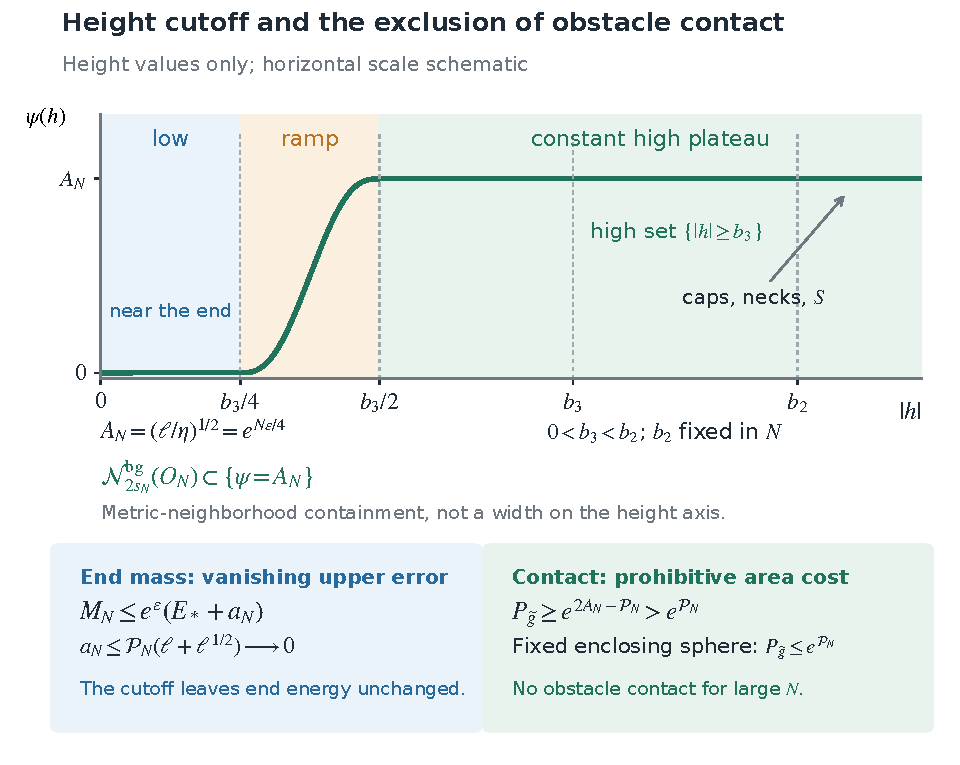
\includegraphics[width=\linewidth]{figures/height-bands.pdf}
 \caption{One admissible height cutoff and its two quantitative effects.  The
 horizontal axis records height values on a schematic scale.  The
 constant plateau $\psi=A_N$ contains the high set $\{|h|\ge b_3\}$
 and the entire further $2s_N$ background neighborhood of its enlarged
 obstacle $O_N$.  Caps, necks, and $S$ lie beyond the fixed threshold
 $b_2>b_3$.  The cutoff vanishes near infinity, while the
 comparison-mass upper error tends to zero.  Any contact of a
 perimeter minimizer with $O_N$ would force total perimeter at least
 $e^{2A_N-\mathcal P_N}$, exceeding the $e^{\mathcal P_N}$ bound
 supplied by a fixed enclosing sphere for large $N$.  The neighborhood
 inclusion is a metric statement, independent of the schematic
 height-axis spacing.}
 \label{fig:cp-height-bands}
\end{figure}

\begin{lemma}[The minimizing frontier avoids the obstacle]
\label{cp:contact-exclusion}
For all large $N$ there is a bounded finite-perimeter set $B_N$
containing $O_N$ whose full $\widetilde g$-perimeter is minimal among
all such bounded sets.  After filling bounded complementary pockets,
its entire frontier $\Gamma_N^0$ is a nonempty compact smooth embedded
minimal surface, disjoint from $O_N$, and its exterior is connected.
Moreover
\begin{equation}\label{cp:competitor-bound}
 P_{\widetilde g}(B_N)\le e^{\mathcal P_N}.
\end{equation}
\end{lemma}

\begin{proof}
Choose a fixed original coordinate sphere beyond the radius containing
$\{|h|\ge b_3/4\}$ and beyond a fixed further neighborhood.  It encloses
$O_N$ for all large $N$ and lies where $\psi=0$.  Its area in
$e^{2(t+\epsilon)}(g+l^2df^2)$ is at most $e^{\mathcal P_N}$ by
Equation~\eqref{cp:quantitative-inputs}.  This proves the proposed
upper bound for the infimum with a radius independent of $N$.

We justify compactness separately at fixed $N$.  Strong asymptotic
flatness gives, sufficiently far out, a foliation by spheres with
positive definite outward second fundamental form.  Follow their
unit-normal trajectories, parametrized by the radius.  Tangential
metrics increase along these trajectories.  Projection from an outer
leaf to an inner leaf consequently contracts two-dimensional area.
For almost every sufficiently large radius $R$, clipping a bounded
competitor at that leaf does not increase its perimeter: along each
normal trajectory where clipping creates boundary, the bounded
competitor must exit farther out; projection of that portion of its
old boundary covers the new trace, with area counted with
multiplicity.  BV slicing and the area formula give the same
inequality for finite-perimeter competitors.  Thus the infimum over
all bounded competitors equals the infimum in one fixed sufficiently
large compact truncation.  BV compactness and lower semicontinuity
\cite[Theorem~3.23 and Proposition~3.6]{AmbrosioFuscoPallara2000}, and
the closed containment condition $B\supset O_N$ almost everywhere
give a minimizer.  Since it minimizes among all bounded competitors,
the outer truncation imposes no local constraint.  Large
mean-convex spheres also exclude a free minimal contact with that
outer truncation.

We prove that the perimeter support has no contact with $O_N$.
Write
\[
 \gamma_N=e^{2(t+\epsilon)}\bar g.
\]
On the $2s_N$-neighborhood of $O_N$, the plateau is constant, and
\begin{equation}\label{cp:plateau-comparison}
 \widetilde g=e^{2A_N}\gamma_N,
 \qquad g_N\le\gamma_N\le L_N^2 g_N,
 \qquad 1\le L_N\le e^{\mathcal P_N}.
\end{equation}
Only pointwise metric comparison is asserted here.

Suppose $q\in O_N\cap\operatorname{supp}|D\mathbf1_{B_N}|$.
Because $B_N$ contains $O_N$ almost everywhere, such a point is in
$\partial O_N$.  Take a shortest background geodesic of length $s_N$
from $q$ to $H_N$.  The ball of radius $s_N/4$ about its midpoint lies
in $O_N\cap B_{s_N}(q)$.  Uniform local background geometry gives
\begin{equation}\label{cp:filled-density}
 |B_N\cap B_{s_N}(q)|_{g_N}\ge c s_N^3.
\end{equation}

We obtain a lower bound for the complementary volume without using
regularity of either frontier.  Put
$v(r)=|B_r(q)\setminus B_N|_{g_N}$ for $0<r<s_N$.
Full minimality against $B_N\cup B_r(q)$, cancellation outside the
ball, and removal of the constant factor $e^{2A_N}$ imply, for almost
every $r$,
\begin{equation}\label{cp:one-sided-perimeter}
 P_{g_N}(B_N;B_r(q))
 \le P_{\gamma_N}(B_N;B_r(q))
 \le L_N^2v'(r).
\end{equation}
The last derivative is the background area of the complementary
trace on the sphere, by coarea.  In the uniform normal charts,
background metric balls correspond to Euclidean balls and volume
and perimeter are uniformly comparable.  Thus the Euclidean
absolute and relative isoperimetric inequalities
\cite[Theorem~3.46 and Remark~3.50]{AmbrosioFuscoPallara2000}
hold here with uniform constants.  Local absolute isoperimetry for
$B_r(q)\setminus B_N$, including its boundary on the sphere, gives
\[
 v(r)^{2/3}
 \le C\bigl(P_{g_N}(B_N;B_r(q))+v'(r)\bigr)
 \le C(L_N^2+1)v'(r).
\]
Every ball at a point of perimeter support has positive complementary
volume.  Integrating the resulting inequality for $v^{1/3}$ from
$\delta$ to $r$ and then letting $\delta\downarrow0$ yields
\begin{equation}\label{cp:unfilled-density}
 v(r)\ge c(L_N^2+1)^{-3}r^3.
\end{equation}
Relative isoperimetry in $B_{s_N}(q)$, together with
Equations~\eqref{cp:filled-density} and~\eqref{cp:unfilled-density},
therefore forces
\[
 P_{g_N}(B_N;B_{s_N}(q))
       \ge c(L_N^2+1)^{-2}s_N^2.
\]
Restoring the constant area multiplier in
Equation~\eqref{cp:plateau-comparison} gives
\begin{equation}\label{cp:contact-area}
 P_{\widetilde g}(B_N)
 \ge e^{2A_N}c(L_N^2+1)^{-2}s_N^2
 \ge\exp(2e^{N\epsilon/4}-\mathcal P_N).
\end{equation}
For fixed $\epsilon>0$, this contradicts
Equation~\eqref{cp:competitor-bound} when $N$ is large.

The minimizing frontier is now disjoint from the obstacle.  It is
locally perimeter minimizing without a constraint and is therefore
smooth and embedded by three-dimensional perimeter regularity
\cite[Regularity Theorem~1.3(iii)]{HuiskenIlmanen2001}.
Filling every bounded complementary pocket cannot increase perimeter
and preserves the obstacle condition.  The frontier of the remaining
exterior is the whole smooth minimal boundary incident on the end.
It is nonempty because a bounded set containing the nonempty open
obstacle cannot have zero perimeter in the connected filled
manifold.  This proves all assertions.
\end{proof}

\subsection{The Riemannian comparison and the limit}

\begin{proposition}[Charged comparison exterior]\label{cp:charged-comparison}
For each fixed strict prepared exterior, each $\epsilon>0$, and all
sufficiently large $N$, there is a smooth one-ended exterior
$\widetilde\Omega_N\subset\operatorname{int}\Omega$, complete with
its compact smooth boundary $\Gamma_N$ included, with the following
properties.  Its metric and fields are the restrictions of the
comparison objects above; the boundary is outermost minimal, and
\begin{align}
 \widetilde g&\ge g,
 &\Area_{\widetilde g}(\Gamma_N)&\ge a_g(S),
       \label{cp:comparison-area}\\
 \operatorname{div}_{\widetilde g}\widetilde{\EE}
 &=\operatorname{div}_{\widetilde g}\widetilde{\BB}=0,
 &R_{\widetilde g}&\ge
   2\bigl(|\widetilde{\EE}|_{\widetilde g}^2
          +|\widetilde{\BB}|_{\widetilde g}^2\bigr).
       \label{cp:comparison-dec}
\end{align}
Its total charges are $Q_E,Q_B$.  Its metric is $O_2(r^{-1})$
asymptotically flat, its fields are $O_1(r^{-2})$, and its scalar
curvature is integrable.  Its ADM mass satisfies
$M_N\le e^\epsilon(E_*+a_N)$ with the error in
Equation~\eqref{cp:mass-error}.
\end{proposition}

\begin{proof}
Apply Lemma~\ref{cp:outermost-enclosure} to the exterior of
$\Gamma_N^0$ from Lemma~\ref{cp:contact-exclusion}.  The comparison
end is strongly asymptotically flat, so its large coordinate spheres
have positive outward mean curvature and confine compact minimal
surfaces by the maximum principle at a largest-radius point.  We
obtain an outermost full minimal enclosure $\Gamma_N$ and take its
exterior $\widetilde\Omega_N$.

The obstacle contains every cap and a neighborhood of the entire
original boundary.  Both $\Gamma_N^0$ and its outer enclosure are
therefore full cuts in the original exterior, with every component
counted.  Their surviving exterior is disjoint from
$H_N=\{|h|\ge b_3\}$.  Lemmas~\ref{cp:curvature}
and~\ref{cp:flux-projection} consequently apply everywhere on
$\widetilde\Omega_N$, up to its boundary.  No part of a filling is
retained.  The construction supplies smoothness, completeness with
boundary, one end and the stated asymptotics.  Finally, metric
dominance on each tangent two-plane and the full-cut definition give
\[
 \Area_{\widetilde g}(\Gamma_N)
 \ge\Area_g(\Gamma_N)\ge a_g(S),
\]
and Equation~\eqref{cp:comparison-mass} gives the mass bound.
\end{proof}

\begin{proposition}[Numerical inequality on a prepared rest exterior]
\label{cp:numerical-prepared}
The strict prepared rest data satisfy
\begin{equation}\label{cp:prepared-inequality}
 E_*\ge Q,
 \qquad
 \sqrt{\frac{a_g(S)}{4\pi}}
      \le E_*+\sqrt{E_*^2-Q^2}.
\end{equation}
This conclusion allows a different fixed choice of future or past
boundary sign on each component.
\end{proposition}

\begin{proof}
Put $r_*=(a_g(S)/(4\pi))^{1/2}$.  We prove the family of bounds
\begin{equation}\label{cp:flux-family}
 E_*\ge sQ+\frac{1-s^2}{2}r_*\qquad(0<s<1).
\end{equation}
The numerical input is the neutral enclosing-area theorem
\cite[Definitions~1.1--1.2 and Theorem~1.3]{NeutralEnclosingArea2026}.
In dimension three it states that a smooth connected oriented complete
one-ended exterior with nonempty compact boundary, integrable neutral
constraint densities satisfying $\mu\ge|J|$, finite future-timelike ADM
vector, decay $g-\delta=O_6(r^{-q_0})$, $K=O_5(r^{-1-q_0})$ for some
$1/2<q_0<1$, and weakly future-trapped boundary on every component obeys
$m\ge\tfrac12(a/(4\pi))^{1/2}$ when its full-cut infimum $a$ is positive.
We verify this contract for the auxiliary data constructed below.

\paragraph{Retained curvature and a flux form.}
Work on the same filled manifold at fixed $\epsilon,N$, and put
\[
 z=t+\epsilon,\qquad g_b=e^{2z}\bar g.
\]
Then $z\ge0$, $g_b\ge g_N$, and
$|dh|_{\bar g}\le\eta/l\le\ell^{1/2}$.  Rotate the two original
fields by the constant matrix $\mathsf R$ in the proof of
Lemma~\ref{cp:flux-projection}, and retain
$\alpha=\iota_{X_e}dV_g$.  It is closed on the original exterior and
has flux $4\pi Q$.  For $Q=0$ the identity rotation suffices.
Extend $\alpha$ smoothly into the filling, cutting it off on fixed
collars inside the original boundary; denote the extension by
$\alpha_{\rm ext}$.  It need not be closed there.  Define
\[
 \iota_{E_b}dV_{g_b}=\alpha_{\rm ext},\qquad
 \iota_{E_{\rm ext}}dV_{g_N}=\alpha_{\rm ext}.
\]
The second field is uniformly bounded on the fixed filling collars,
is $O_1(r^{-2})$ on the end, and has $L^2$ and $L^6$ norms bounded
polynomially in $1+N$.  On the original exterior $E_b$ is divergence
free.  The square completion in
Equations~\eqref{cp:projection-square}--\eqref{cp:two-form-norm} gives
\[
 e^{2z}|E_b|_{g_b}^2=e^{-2z}|\alpha|_{\bar g}^2
 \le I_g(w).
\]

We need a sharper consequence of the existing quadratic identity:
\begin{equation}\label{cp:sharp-gradient}
 \mathcal T\ge\frac34|dt|_{A_d}^2.
\end{equation}
Here is a direct check.  In Equation~\eqref{sy:positive-squares},
minimize over $M,F,j$, keeping the transverse and axial components
$y,x$ of $dt$ fixed.  The transverse coefficient is
$2s_p-v/4\ge3/4$.  The remaining axial coefficient, divided by $d$, is
\[
 C(p,v)=\frac{(2p+1)(8+v)}{8+4v+6pv}.
\]
This is increasing in $p\ge0$, and
$C(0,v)=(8+v)/(8+4v)\ge3/4$ for $0\le v<1$.
This proves Equation~\eqref{cp:sharp-gradient}, including zero slope
by the invariant definition of $\mathcal T$.

Let $\mathcal U_N$ be the part of the original exterior where
$|h|\le b_3$.  Equation~\eqref{cp:unmodified-curvature} and
$\delta_0<1/24$ show that throughout $\mathcal U_N$,
$R_{g_b}/2\ge|E_b|_{g_b}^2$.  On the fixed original band
$b_3/4\le|h|\le b_3$, the positive function $\rho$ has a fixed
positive lower bound $c_*$; hence, since
$(1-\delta_0)3/4>2/3$, we have the stronger bound
\begin{equation}\label{cp:retained-band}
 e^{2z}R_{g_b}/2\ge e^{2z}|E_b|_{g_b}^2+c_*
                       +\frac23|dt|_{\bar g}^2.
\end{equation}
The end estimates already proved give all-order decay
$g_b-\delta=O_j(r^{-1})$ after the constant dilation, integrable
scalar curvature, and
\[
 E(g_b)\le e^\epsilon(E_*+a_N),\qquad a_N\longrightarrow0.
\]

\paragraph{A smooth bounded flux profile.}
Fix $s\in(0,1)$ and write $y_0=\log(1-s^2)<0$.  For every
$t_0>0$ choose smooth functions $L>0$ and $H_0$ on the real line with
\begin{gather*}
 L(0)=1,\qquad L'\ge0,\qquad
 H_0=0\ \hbox{on }(-\infty,y_0],\qquad
 \operatorname{supp}H_0'\Subset(y_0,0),\qquad H_0'\ge0,\\
 |H_0'|\le2\sqrt{1+2L'/L}\,e^yL,
 \qquad 2s-t_0<H_0(0)\le2s.
\end{gather*}
To construct them, set $c=1-s^2$ and first use
$L_{\rm opt}(y)^2=(1-ce^{-y})/s^2$ for $y>y_0$.
The right side in the bound for $H_0'$ is then $2e^y/s$, whose
integral from $y_0$ to zero is $2s$.  For a small $\sigma>0$, replace
$L_{\rm opt}'$ below $y_0+\sigma$ by
$\chi_\sigma L_{\rm opt}'$, where $\chi_\sigma$ is nondecreasing,
zero below $y_0+\sigma/3$, and one above $y_0+2\sigma/3$; integrate
backwards from the unchanged value at $y_0+\sigma$.
This gives a positive smooth nondecreasing $L$ on the whole line,
constant at its lower end.  Take $H_0'=\zeta_\sigma\,2e^y/s$,
where $0\le\zeta_\sigma\le1$ is smooth and supported in
$(y_0+\sigma,-\sigma)$ and tends to one on $(y_0,0)$.
Put $H_0(y)=\int_{-\infty}^yH_0'(v)\,dv$ and decrease $\sigma$
until the asserted value at zero holds.

Define $B(0)=0$, $B'(y)=e^yL(y)$.  This is strictly increasing,
its range on $[y_0,\infty)$ is $[B(y_0),\infty)$, and
$B(y)\ge e^y-1$ for $y\ge0$.  Set $Y_0=B(y_0)<0$ and extend
\[
 \mathfrak h(Y)=H_0(B^{-1}(Y))\quad(Y\ge Y_0),\qquad
 \mathfrak h(Y)=0\quad(Y<Y_0).
\]
This is smooth and bounded, vanishes near and below $Y_0$, and is
constant for all sufficiently large $Y$.

\paragraph{The second scalar solve.}
There is a smooth solution on the entire filled manifold of
\begin{equation}\label{cp:bounded-flux-equation}
 2\Delta_{g_b}B(y)=\operatorname{div}_{g_b}(H_0(y)E_b),
 \qquad y\longrightarrow0\quad\hbox{at infinity},
 \qquad y\ge y_0.
\end{equation}
We supply the estimates needed for this assertion; no estimate
uniform in $s$ or in the profile tolerance is required.
Set $Y=B(y)$.  In the background measure its equation is exactly
\begin{equation}\label{cp:background-flux-equation}
 2\operatorname{div}_{g_N}(A\nabla Y)
   =\operatorname{div}_{g_N}(\mathfrak h(Y)E_{\rm ext}),
 \qquad A=e^z\sqrt D\,A_d.
\end{equation}
Indeed the volume ratio is $e^{3z}\sqrt D$, and its product with
$E_b$ is $E_{\rm ext}$.  The axial and transverse eigenvalues of
$A$ are $e^z/\sqrt D$ and $e^z\sqrt D$; thus their upper bounds
and positive inverse lower bounds are at most $\exp(\mathcal P_N)$.

The filled background has the Sobolev inequality
\[
 \|v\|_6^2\le S_N\|dv\|_2^2,
 \qquad S_N\le\exp(\mathcal P_N),
\]
for compactly supported $v$, with the same bound on every outer
truncation with zero trace.  To verify the dependence on $N$, cover
the compact core and its product necks by $O(1+N)$ uniformly
controlled patches with bounded overlap.  Chains of at most
$O(1+N)$ overlapping patches join them to a fixed end annulus.
Radial integration from infinity controls the annulus's $L^2$
norm by the end gradient energy, because
$\int_R^\infty r^{-2}\,dr<\infty$.  Local Poincar\'e inequalities
control the successive differences of patch averages.  Summing
along the chains bounds the core $L^2$ norm by a polynomial
multiple of the global gradient energy.  The local Sobolev
inequalities and the Euclidean end inequality then give the
stated bound.

Solve Equation~\eqref{cp:background-flux-equation} on expanding
smooth outer truncations with zero Dirichlet data.  Multiplying
its right side by any homotopy parameter in $[0,1]$ leaves the
following estimates unchanged.  The vector
$F_Y=\mathfrak h(Y)E_{\rm ext}$ has bounded $L^2$ and $L^6$ norms,
independent of $Y$ and of the outer radius.  Testing by $Y$ gives
$\|dY\|_2+\|Y\|_6\le\exp(\mathcal P_N)$.
For $a>0$, test by $(Y-a)_+$.  H\"older and Sobolev give
\[
 \|(Y-a)_+\|_6\le C_N|\{Y>a\}|^{1/3},
 \qquad C_N\le\exp(\mathcal P_N).
\]
For $b>a$ this implies
\[
 |\{Y>b\}|\le
 \left(\frac{C_N}{b-a}\right)^6|\{Y>a\}|^2.
\]
Starting at level one, whose superlevel measure is bounded by the
energy estimate, and taking levels $1+d_*(1-2^{-j})$ proves
$\sup Y\le\exp(\mathcal P_N)$ for a sufficiently large
$d_*\le\exp(\mathcal P_N)$.  The identical argument for negative
levels bounds $\inf Y$.

On a fixed truncation, freezing $F_Y$ and solving the linear
uniformly elliptic Dirichlet equation defines a continuous compact
map on the continuous functions with zero boundary values:
linear $W^{1,p}$ estimates with $p>3$ give compactness.
The preceding bounds hold for every fixed point of its homotopy
with zero.  Leray--Schauder degree therefore gives a fixed point.
Divergence-form local H\"older estimates, then divergence Schauder
estimates and differentiation, make it smooth.  The same estimates
are uniform on each fixed compact subset as the truncation radius
tends to infinity, so a diagonal limit solves the equation on the
filled manifold.  These are the standard uniformly elliptic
Dirichlet and interior estimates
\cite[Chapters~6--8]{GilbargTrudinger2001}.
Testing by $(Y_0-Y)_+$ gives zero gradient, since
$\mathfrak h=0$ on its support and its outer trace vanishes.
Consequently $Y\ge Y_0$ both on each truncation and in the limit.
Inverting $B$ proves $y\ge y_0$ and, from its exponential growth,
$y\le\mathcal P_N$.

On the original end $\operatorname{div}_{g_b}E_b=0$, so
$2\Delta_{g_b}Y=\mathfrak h'(Y)E_b(Y)$, with bounded drift
$O(r^{-2})$.  For fixed $0<\beta'<1$, positive multiples of
$r^{-1}(1-r^{-\beta'})$ are supersolutions of the absolute drift
comparison equation outside a fixed radius.  Their negative
Laplacian has order $r^{-3-\beta'}$, which dominates the metric
error and drift terms of order $r^{-4}$.  Comparison with both
signs and the zero data at each outer boundary proves
$Y=O(r^{-1})$ uniformly during exhaustion.  Scaled estimates give
the first two derivative orders.  Thus $y\to0$ and eventually
$H_0(y)=H_0(0)$; on that end $Y$ is harmonic.  The all-order metric
bounds then give $Y,y=O_j(r^{-1})$ for every fixed $j$.
Integration on the whole filled truncation, which has no inner
boundary, gives the exact limiting flux
\begin{equation}\label{cp:conversion-flux}
 \lim_{R\to\infty}\int_{S_R}\partial_{\nu_b}y\,dA_{g_b}
       =\frac{H_0(0)}2\,4\pi Q.
\end{equation}
Indeed the flux identity first holds with $Y$ in place of $y$;
$B'(0)=1$ and the $O_j(r^{-1})$ decay make their difference tend
to zero.  This also explains why source terms in the artificial
filling impose no omitted inner flux condition.

\paragraph{A neutral exterior.}
Set $\gamma=e^{2y}g_b$.  On $\mathcal U_N$, expansion of the
scalar equation and the conformal curvature identity give
\begin{align*}
 e^{2y}R_\gamma/2
 &\ge |E_b|^2-
 \frac{H_0'}{e^yL}E_b(y)
       +(1+2L'/L)|dy|_{g_b}^2\ge0.
\end{align*}
The last inequality is precisely the profile discriminant bound.
On the band, the terms in Equation~\eqref{cp:retained-band}
beyond the field norm remain available.  Moreover, when $y\ge0$
one has $H_0'=0$, so the full additional $|dy|^2$ term is retained.
Therefore
\begin{equation}\label{cp:neutral-band}
 e^{2(z+y)}R_\gamma/2\ge c_*+\frac23|dt|_{\bar g}^2
             +\mathbf1_{\{y\ge0\}}|dy|_{\bar g}^2.
\end{equation}
Everywhere on the filled manifold
$\gamma\ge e^{2y_0}g_N$.  The conformal ADM calculation, with
normalizing factor $1/(16\pi)$, and
Equation~\eqref{cp:conversion-flux} give
\begin{equation}\label{cp:conversion-mass}
 e_N:=E(\gamma)=E(g_b)-\frac{H_0(0)}2Q.
\end{equation}
The metric has all-order $O(r^{-1})$ decay.  Its scalar curvature
is integrable: far out $B(y)$ is harmonic, so
$\Delta_{g_b}y=-(1+L'/L)|dy|^2=O(r^{-4})$, and $R_{g_b}$ is
integrable.

Choose a fixed smooth function $b$ with $b=0$ on $(-\infty,0]$,
$0\le b'\le1$, and $b'=1$ for all sufficiently large arguments.
Then $C(y)=e^{y-b(y)}$ is bounded above and below by positive
constants on $[y_0,\infty)$.  We shall use a compactly supported
pure-trace tensor
\[
 K'=-a\gamma,\qquad
 a=e^{-z-b(y)}\mathcal H(|h|),
\]
where $\mathcal H$ vanishes on $[0,b_3/4]$ and is a constant $M$
on $[b_3/2,b_3]$.  For such a tensor the neutral densities are
$\mu'=R_\gamma/2+3a^2$ and $J'=2\,da$.
Multiplication by $e^{2(z+y)}$ bounds its momentum contribution by
\[
 2C\left(\mathcal H|dt+b'dy|_{\bar g}
             +\frac\eta l|\mathcal H'|\right).
\]
Young's inequality absorbs the first term into the two gradient
terms of Equation~\eqref{cp:neutral-band} at a cost at most
\[
 C^2\mathcal H^2\left(\frac{1}{2/3}+1\right)
       =\frac52C^2\mathcal H^2.
\]
Where $y<0$, $b'=0$, so no unavailable $y$-gradient term is used.
The remaining energy coefficient is $3-5/2=1/2>0$.
Consequently the neutral DEC follows if
\[
 \frac\eta l|\mathcal H'|\le c'(1+\mathcal H^2)
\]
for a fixed sufficiently small $c'>0$, depending only on $c_*$
and the two bounds for $C$.  This condition can be enforced for
\emph{every finite} plateau $M$ by a single sufficiently large $N$:
choose a fixed smooth cutoff $\chi_h$ from zero to one between
$b_3/4$ and $b_3/2$, and set
\[
 \mathcal H(v)=\tan((\arctan M)\chi_h(v)).
\]
Then $|\mathcal H'|/(1+\mathcal H^2)\le
(\pi/2)\|\chi_h'\|_\infty$ independently of $M$, whereas
$\eta/l\le\ell^{1/2}\to0$.  Its composition with $|h|$ is smooth
because it vanishes on a neighborhood of zero.

After these scalar solves, choose a regular value
$c_h\in(b_3/2,b_3)$ of $|h|$.  Let $\mathcal D_N$ be the closure
of the component of $\{|h|<c_h\}$ containing the end.
The height gap keeps it entirely in the original exterior.
Its full boundary is compact, smooth, embedded, two-sided and
nonempty.  Since this boundary is fixed and compact, take the
plateau $M$ sufficiently large that, with normal toward the end,
\[
 H_{\partial\mathcal D_N}+
      \operatorname{tr}_{\partial\mathcal D_N}K'
       =H_{\partial\mathcal D_N}-2a<0
\]
on every component.  The choice of $N$ need not be changed when
$M$ is chosen.  Restrict $\gamma,K'$ to $\mathcal D_N$.
They are smooth, satisfy the neutral DEC, and $K'$ is compactly
supported.  This is a connected oriented one-ended exterior with
compact complement of its coordinate end.  It is complete with
boundary: its domain is closed in the original complete exterior,
and its metric is bounded below by $e^{2y_0}g$.
All-order metric decay and compact support of $K'$ imply the
neutral theorem's $O_6/O_5$ assumptions for any $1/2<q_0<1$.
The densities are integrable and its momentum is zero.

Every full cut in $\mathcal D_N$ is a full cut of the original
exterior.  Counting all components and contact portions, the metric
comparison therefore gives its full-cut infimum $a_N'$ the bound
\[
 a_N'\ge e^{2y_0}a_g(S)>0.
\]
If $e_N\le0$, use the energy-raising conformal family constructed
in the proof of Lemma~\ref{en:timelike-reduction}, with zero fields
and with its radial function constant on a core containing
$K'$ and the boundary.  The neutral DEC and trapping persist,
areas do not decrease, momentum remains zero, and the energy
becomes $e_N+2\lambda$.  The all-order end decay persists for this
radial construction.  For arbitrarily small $e>0$, choose
$\lambda=(e-e_N)/2$.  The neutral theorem would imply
$e\ge\tfrac12e^{y_0}r_*>0$, a contradiction.
Thus $e_N>0$, and applying that theorem directly gives
\[
 e^\epsilon(E_*+a_N)-\frac{H_0(0)}2Q
      \ge\frac12e^{y_0}r_*=
                    \frac{1-s^2}{2}r_*.
\]
At fixed prepared data, $s$, profile, and $\epsilon$, let
$N\to\infty$.  Then let $\epsilon\downarrow0$ and finally
$t_0\downarrow0$.  This proves Equation~\eqref{cp:flux-family}.
No convergence of comparison horizons or uniform estimate at
$s=0,1$ is required.

Letting $s\uparrow1$ first yields $E_*\ge Q$.
If $r_*>Q>0$, choose $s=Q/r_*$ to get
$E_*\ge(r_*+Q^2/r_*)/2$; for $Q=0$ the same conclusion follows
by $s\downarrow0$.  Since $r_*>Q$, this is equivalent to
$r_*\le E_*+\sqrt{E_*^2-Q^2}$.  If $r_*\le Q$, that upper-radius
bound follows directly from $E_*\ge Q$.  This proves both
assertions of Equation~\eqref{cp:prepared-inequality}.
The original componentwise signs enter only in the height-gap
construction.  Every component of the new auxiliary boundary has
the common future sign required by the neutral theorem.
\end{proof}

\begin{proof}[Proof of Theorem~\ref{thm:numerical}]
First suppose the original ADM vector is future timelike, and write
$m=\sqrt{E^2-|P|^2}$.  Proposition~\ref{en:rest-preparation} supplies
strict prepared rest exteriors indexed by $j$ with
\[
 E_{*,j}\longrightarrow m,\qquad
 (Q_{E,j},Q_{B,j})=(Q_E,Q_B),\qquad
 a_{g_j}(S)\longrightarrow a_g(S).
\]
The area convergence is for the full original cut class.  More
explicitly, the lower metric comparison
$g_j\ge(1-\delta_j)g$, with $\delta_j\to0$, gives
$a_{g_j}(S)\ge(1-\delta_j)a_g(S)$; local smooth convergence on any
fixed full cut gives the reverse upper limit after taking its area
arbitrarily close to the infimum.  Thus no original minimizing cut
is needed.  The preparation keeps the fixed sign on each boundary
component.

For each $j$, Proposition~\ref{cp:numerical-prepared} has already
taken the limits in the order: outer Dirichlet exhaustion at fixed
$N$, then $N\to\infty$, then $\epsilon\downarrow0$.  Apply its
conclusion and only now let $j\to\infty$.  It follows that
\[
 m\ge Q,\qquad
 r_A\le m+\sqrt{m^2-Q^2}.
\]
Since $E>0$, the first inequality is equivalent to
$E\ge\sqrt{|P|^2+Q^2}$.

Finally, Proposition~\ref{ct:full-cut-positive} gives $a_g(S)>0$ for every
original exterior in the theorem.  We recall explicitly how
Lemma~\ref{en:timelike-reduction} eliminates the remaining ADM
endpoint using the timelike conclusion just proved.  Its conformal
energy-raising family preserves $P,Q_E,Q_B$, the matter condition
and the componentwise boundary signs, increases every full-cut
area, and changes the energy to $E_s=E+2s$.  If $E\le|P|$, take
$s>(|P|-E)/2$.  The family then has a future-timelike ADM vector, so
the preceding result applies and in particular gives
\[
 \sqrt{(E+2s)^2-|P|^2}
 \ge\frac12\sqrt{\frac{a_{g_s}(S)}{4\pi}}
 \ge\sqrt{\frac{a_g(S)}{16\pi}}>0.
\]
Here we used $x+\sqrt{x^2-Q^2}\le2x$ for $x\ge Q$.  Letting
$s\downarrow(|P|-E)/2$ makes the left side tend to zero, a
contradiction.  Hence $E>|P|$ in the original data.  The already
proved timelike case completes the theorem, with no boost of speed
one and no additional area or timelikeness hypothesis.
\end{proof}
